\chapter{Metodología}
	
En los capítulos anteriores se ha presentado los distintos algoritmos de control y generación de trayectorias que se emplearán para intentar recorrer un circuito con un cuadricóptero de carreras autónomo en un entorno simulado. En este apartado se presenta la metodología empleada para superar el circuito que fue propuesto durante las pruebas clasificatorias del Alphapilot 2019.

\section{Sistemas de referencia}
Antes de continuar con la metodología empleada, es conveniente fijar los sistemas de referencia que se van a emplear. Primeramente se empleara un sistema de coordenadas global en el mundo. El origen de este sistema de referencia global fijo viene dado por el simulador y se encuentra en el centro del circuito. A partir de este sistema estableceremos el sistema de referencias móvil del aeronave, cuyo origen se encuentra en el centro de masas del cuadricóptero y las direcciones de los ejes siguen el estándar ENU (\textit{East North Up}). Finalmente, se generará un sistema de referencia móvil para cada puerta del circuito, cuyos orígenes corresponderán al centro de las puertas. 

\begin{figure}[htb!]
	\centering
	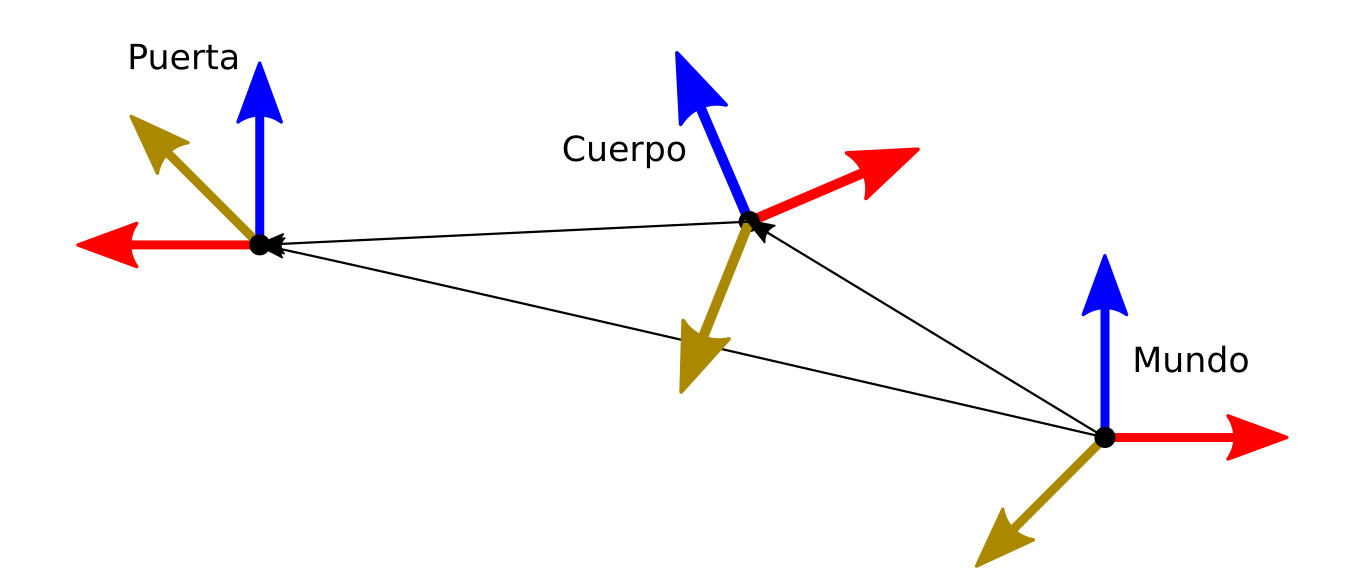
\includegraphics[width=0.75\textwidth]{imagenes/frames}
	\caption{Transformaciones entre los sistemas de referencia de las puertas, el cuerpo del aeronave y el mundo.}
	\label{waypoints:Refs}
\end{figure}



\section{Generación de \textit{waypoints}}
\label{section:gen_traj}
Para recorrer el circuito de forma satisfactoria es necesario que del aeronave atraviese las distintas puertas o \textit{gates} que componen el circuito en un orden concreto. Para conseguir esto es necesario conocer las posiciones de las puertas en el mundo y generar los puntos de paso necesarios para que del aeronave pase a través de ellas sin colisionar.

\begin{figure}[htb!]
	\centering
	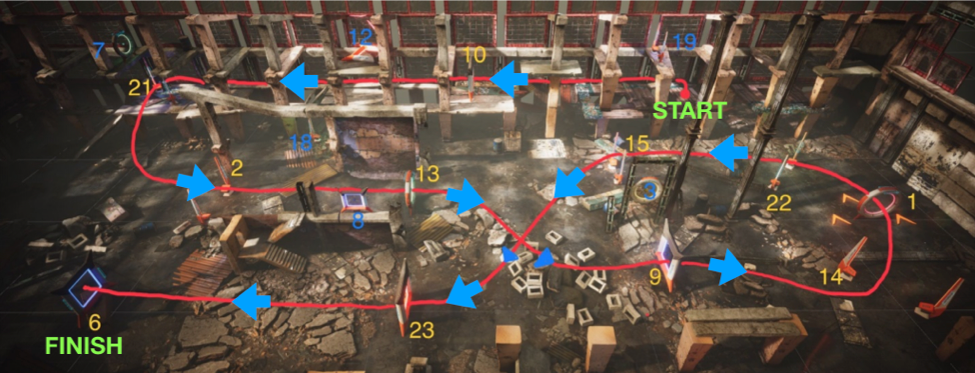
\includegraphics[width=\textwidth]{imagenes/diagramacircuito}
	\caption{Vista aérea del circuito en el simulador FightGoggles, las puertas que se deben traspasar se simbolizan con su número en color amarillo.}
	\label{waypoints:circuito}
\end{figure}

Como se puede observar en la figura \ref{waypoints:circuito} del aeronave debe recorrer 11 puertas, cada una con un número de identificación, en un orden concreto. Cada una de estas puertas posee unas medidas estandarizadas de 2x2 m.

En la competición se proporciona el orden en el que se deben atravesar las puertas y una posición aproximada de las posiciones de cada una de ellas en el mundo. Esta posición aproximada posee un error significativo, por lo que es necesario corregir la estimación de la posición de estas puertas a medida que del aeronave avanza por el circuito (estimación \textit{online}).
\begin{figure}[htb!]
	\centering
	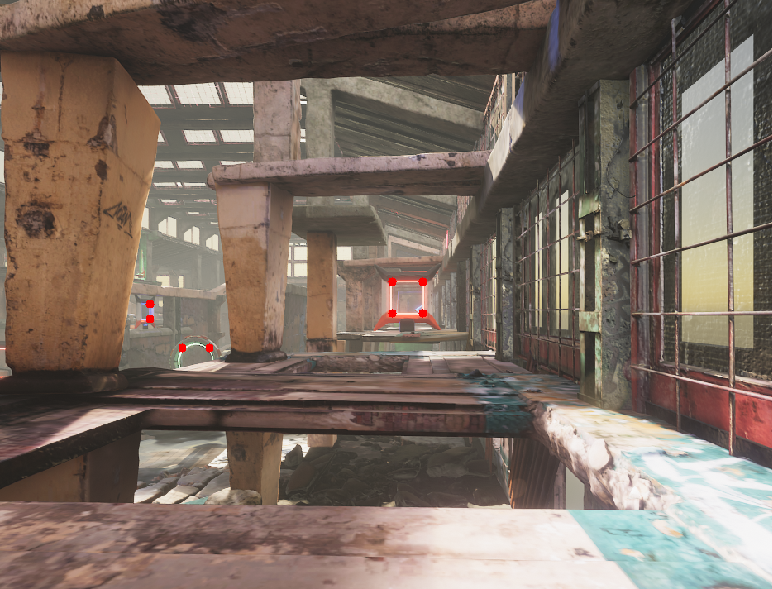
\includegraphics[width=0.68\textwidth]{imagenes/red_points}
	\caption{La imagen provista por el simulador con las esquinas de las puertas visibles marcadas en rojo.}
	\label{redpoints}
\end{figure}


Para poder realizar la estimación \textit{online} de las puertas, es necesario percibirlas, para ello se hace uso de las cámaras integradas en del aeronave simulada. Las cámaras del cuadricóptero permiten localizar las distintas puertas a lo largo del circuito. La imagen provista por el simulador, además de contener la imagen observada por la cámara, contiene también las posiciones en el plano imagen, de las esquinas de las puertas visibles (Figura \ref{redpoints}), así como el identificador de puerta a la que corresponde.



Esta información extra provista por el simulador facilita enormemente la estimación de las posiciones de las distintas puertas, reduciendo también el tiempo de calculo requerido.



Dado que se cuenta con los parámetros físicos de la cámara y con las dimensiones de las puertas, es posible emplear un algoritmo PnP (\textit{Perspective n-Points}) para calcular la posición relativa de los \textit{frames} con respecto a del aeronave. Concretamente, se ha empleado la medida de la posición del centro de la puerta, ya que nos permite generar los waypoints de forma más sencilla.






La incertidumbre de estas medidas disminuye a medida que el aeronave se acerca a las puertas, por lo que cuando las imágenes se toman a una distancia lejana, el error que tienen es elevado. Para disminuir la influencia de las medidas erróneas cada medida se somete a un filtrado en dos pasos:

\begin{enumerate}
	\item \textbf{Región de confianza:} Dado que siempre se posee una posición estimada de cada puerta es posible emplear esta información para descartar medidas erróneas. Siendo $\hat{G_i}$ la estimación previa del centro de la puerta $i$, se establece una bola $B(\hat{G_i},r)$ con centro en $\hat{G_i}$  y radio $r$ como región de confianza, es decir, si una nueva medida $G_i \notin B(\hat{G_i},r)$ entonces se desecha como una medida errónea.
	El valor del radio $r$ influye en la distancia máxima que puede tener una medida respecto a la estimación original para considerarse correcta. Dado que al comienzo del circuito se tienen unas posiciones de las puertas con un error muy grande, este valor $r$ no puede ser muy bajo, si no no se conseguiría corregir la posición de las puertas con mediciones correctas. Por el contrario, si el valor de $r$ es muy grande, este filtrado carecería de sentido, ya que cualquier medición se consideraría válida. En la practica se han probado con distintos valores de este parámetro, obteniendo mejores resultados con valores de $r$ de entre 4 y 6 metros.
	\item \textbf{Media móvil:} Si la medida obtenida $G_i$ se encuentra contenida en esa región, entonces, en lugar de sustituir directamente la estimación de la posición de esta puerta, se realiza una modificación de la medición anterior, de acorde a la fórmula:
	\begin{equation}
		\hat{G_i} = \alpha \hat{G}_{i,prev} + (1-\alpha)G_i
	\end{equation}
	siendo $\hat{G}_{i,prev}$ la estimación anterior y $\alpha \in (0,1)$ un parámetro de filtrado. Cuando $\alpha$ tiene valores pequeños, la estimación cambia rápidamente con las nuevas medidas, mientras que si $\alpha$ posee valores altos, la estimación varía ligeramente con cada una de las nuevas medidas. Los valores que se suelen emplear son $\alpha = 0.9$ y $\alpha = 0.99$. Para este filtrado se ha empleado un valor de $\alpha = 0.9$ dado que presenta un buen equilibrio entre robustez y reactividad ante nuevas medidas.

\end{enumerate}


Con este proceso se consiguen actualizar las posiciones estimadas de las puertas con una frecuencia aproximada de 60 Hz, la frecuencia de refresco de las cámaras. En los casos en los que se encuentran varias puertas en la imagen se realizan el filtrado anterior para cada una de ellas por separado.

\section{Trayectorias a largo y corto plazo}

Con la posición estimada de cada puerta en el mundo es posible construir la trayectoria que el dron debe seguir para completar el circuito. El problema es que estas posiciones cambian continuamente, siendo más fiables cuanto más cerca se encuentre el aeronave de la puerta, por lo que es necesario actualizar estas trayectorias de la forma mas ágil posible. Para conseguir que el sistema sea capaz de reaccionar de forma fluida a los cambios en la estimación de las puertas, se ha dividido la generación de trayectorias en dos partes : una a largo plazo que tiene en cuenta las posiciones de las puertas y una a corto plazo que genera trayectorias óptimas en un horizonte temporal finito.

Dado que el circuito es amplio y no existen obstáculos entre dos puertas sucesivas, no se tienen en cuenta los obstáculos del circuito para la generación de trayectorias. Para asegurar esto, es necesario que las trayectorias generadas no se alejen demasiado de las lineas rectas que unen las distintas puertas sucesivas. A continuación, se explicará de forma más detallada cómo se generan estas trayectorias.
\subsection{Trayectoria a largo plazo}

Para poder generar trayectorias suaves a lo largo de todo el circuito es conveniente tener en cuenta las posiciones aproximadas de todas las puertas,  de esta forma a medida que el aeronave recorre la trayectoria obtiene nuevas estimaciones que permiten ir refinando la trayectoria. Si se generase la trayectoria solo teniendo en cuenta los $m$ siguientes waypoints, la trayectoria a seguir variaría mucho después de pasar una puerta, lo que perjudicaría en el rendimiento del aeronave. Dado que el dron obtiene nuevas mediciones a una frecuencia de unos 60 Hz esta trayectoria se tiene que ir actualizando continuamente, por lo que es conveniente minimizar el tiempo de cómputo de cada una. 

Como se ha presentado en el capítulo \ref{cap:gen_tray} las trayectorias que se van a emplear son \textit{splines} en las que el grado de los segmentos polinómicos depende de la acción de control a minimizar. Los dos factores que afectan principalmente al tiempo de cómputo son el grado de los segmentos polinomiales, ya que a mayor grado, mayor número de coeficientes se deben calcular, y el número de \textit{waypoints}, ya que aumenta el número de segmentos polinomiales.

Para poder generar una ruta a través de todo el circuito que se calcule de la forma más rápida posible y que tenga en cuenta las limitaciones físicas del aeronave, se ha empleado trayectorias de aceleración mínima ($n = 2$) con 12 \textit{waypoints}, 11 de las puertas y 1 de la posición del aeronave. Estas trayectorias son rápidas de calcular y permiten actualizar la trayectoria con una frecuencia superior a la de adquisición de la cámara. Estas trayectorias cambian continuamente, por lo que no es conveniente usar estas trayectorias para controlar el cuadricóptero ya que las referencias del controlador estarían cambiando continuamente, generando un movimiento muy poco fluido. Para solucionar esto se emplean las trayectorias a corto plazo.

\begin{figure}[htb!]
	\centering
	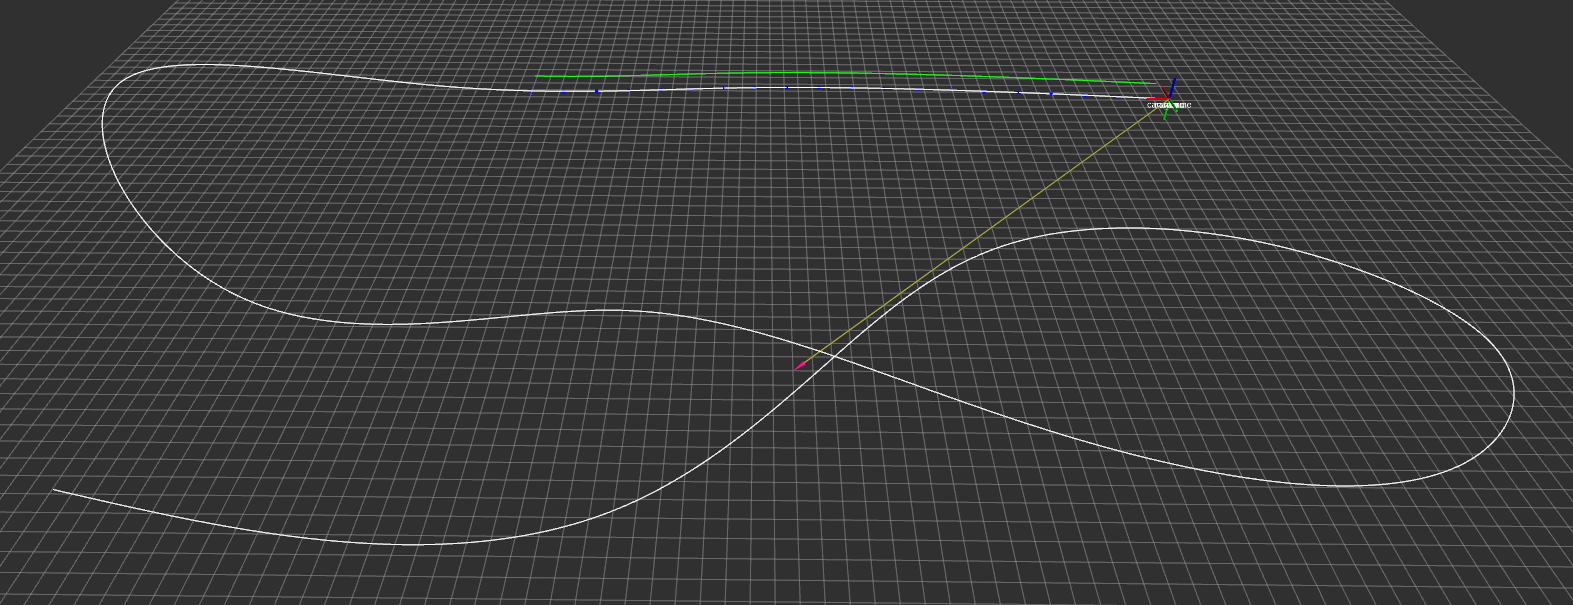
\includegraphics[width=1\textwidth]{imagenes/Rviz_traj_largo}
	\caption{Visualización de las trayectoria a largo (blanco) y a corto (verde) plazo en Rviz.}
	\label{rviz:traj_largo}
\end{figure}
\newpage

\subsection{Trayectoria a corto plazo}

Para generar la trayectoria que va a seguir el controlador, es conveniente generar trayectorias de \textit{snap} mínimo ($n=4$), ya que son las que generan trayectos más suaves. El grado de los polinomios que componen estas \textit{splines} son de grado 7, lo que implica un elevado coste computacional. Además, es conveniente que los \textit{waypoints} empleados para generar esta trayectoria estén cerca (una distancia inferior a los 8 m entre waypoints), ya que si se eligen waypoints muy separados, la trayectoria resultante puede separarse demasiado de la linea recta entre ellos, llegando a poder colisionar con el entorno. Por lo que para generar una trayectoria completa del circuito sería necesaria una gran cantidad de waypoints, por lo que el tiempo de cómputo sería muy elevado, haciendo que el sistema no sea capaz de reaccionar a cambios en las posiciones de las puertas de forma rápida.

Para poder conseguir trayectorias de control óptimas se ha decidido partir de la trayectoria a largo plazo y establecer un horizonte temporal, sobre el cual se calcule la trayectoria a corto plazo. Este proceso se genera en varias etapas:
\begin{enumerate}
	\item Se localiza la posición del cuadricóptero dentro de la trayectoria a largo plazo. Para ello se parte de la última posición conocida de el aeronave en la trayectoria $t_c$ y se comprueba en un pequeño intervalo, en que posición se encuentra el aeronave. Dado que el sistema tiene inercia y los algoritmos tardan un tiempo en procesarse, es necesario recalcular esta posición para obtener una mayor precisión.
	
	\item Se muestrea la trayectoria a largo plazo para obtener los waypoints de la trayectoria a corto plazo. Partiendo de la posición obtenida previamente $t_c$, se fija un horizonte temporal en el que se quiere calcular la trayectoria a corto plazo $t_h$, también se fija la distancia a la que se quiere que se encuentren los waypoints $t_d$. Con estos datos se  muestrea la trayectoria en el intervalo $t \in (t_c, t_c + t_h)$ con una distancia de muestreo $t_d$ entre muestras. Las muestras obtenidas constituyen el conjunto de \textit{waypoints} que se emplearán para generar la trayectoria a corto plazo.
	
	\item Finalmente, se genera una trayectoria de \textit{snap} mínimo empleando el conjunto de waypoints obtenidos previamente. La trayectoria obtenida $P(t) :[0,t_f] \rightarrow \mathbb{R}^3$ proporciona las posiciones en el espacio tridimensional en las que deberá estar el cuadricóptero para cada instante de tiempo. Para generar las consignas del controlador es conveniente conocer también las velocidades y acceleraciones para cada instante de tiempo, por lo que se derivan estos splines para obtener la trayectoria en velocidad $V(t) :[0,t_f] \rightarrow \mathbb{R}^3$ y la trayectoria en acceleración  $A(t) :[0,t_f] \rightarrow \mathbb{R}^3$ siendo $t_f$ el tiempo de finalización de la trayectoria.
\end{enumerate}

Para conseguir que estas trayectorias tengan en cuenta los cambios $P(t)$, $V(t)$ y $A(t)$ en la estimación de las puertas, estas trayectorias se recalculan periódicamente a medida que se modifica la trayectoria a largo plazo.

\subsection{Orientación del aeronave en \textit{yaw}}
Además de las referencias de posición en el espacio tridimensional, para controlar el estado del aeronave es necesario indicar el angulo de \textit{yaw} deseado. De cara a obtener las mejores estimaciones en las posiciones de las puertas, se desea que el aeronave siempre este orientada de forma que las camáras miren hacia delante. Partiendo de la trayectoria a corto plazo $V(t)$ es facil obtener el valor requerido del angulo de \textit{yaw} $\psi$. Siendo $v_x(t)$ y $v_y(t)$ las componentes de la trayectoria $V(t)$ para el eje x y el eje y respectivamente, en ángulo de yaw deseado es:

\begin{equation}
	\psi_{des}(t) = -atan2(v_x,v_y) + \pi/2
\end{equation}
siendo $atan2(x,y)$ el arco tangente de dos parámetros entre $x$ e $y$. Con esta simple expresión se consigue que el aeronave se oriente de forma que las cámaras miren hacia donde se va a mover el aeronave.


















